\chapter{Hasil dan Pembahasan}

\section{Pemeriksaan Fungsionalitas di Windows Subsystem for Linux (WSL)}

Sejauh ini, WSL belum memiliki dukungan penampilan notifikasi dan pengontrolan media yang tertampil secara \textit{native} di \textit{shell} Windows. Hal ini dapat diuji dengan perangkat-perangkat lunak yang mendukung penjalanan di Linux dan memanfaatkan notifikasi dan/atau sistem kontrol media universal dalam interaksinya dengan pengguna. Pada aplikasi Spotify yang berjalan di dalam WSL, sebagai contoh, pemutaran media tidak menghasilkan sistem pengontrolan media universal yang biasanya tertampil di bilah pengaturan cepat (\textit{quick settings}) pada Windows 11. Sama halnya dengan penampilan notifikasi; pemanggilan alat \verb|notify-send| di terminal WSL menghasilkan eror yang menyebutkan bahwa belum ada layanan D-Bus yang menangani hal pernotifikasian.

% TODO: Insert screenshots here

\section{Analisis pada Sistem Operasi Linux Sungguhan}

Dengan bantuan perangkat lunak virtualisasi UTM, analisis sistem penanganan notifikasi dan sisten kontrol media pada sistem operasi Linux sungguhan dilakukan pada sebuah \textit{virtual machine} (bertindak sebagai komputer referensi) yang menjalankan sistem operasi Ubuntu 22.04 (LTS) edisi arsitektur ARM 64-bit dan berjalan di atas perangkat komputer \textit{host} MacBook Air keluaran tahun 2020 (berprosesor M1) bersistem operasi macOS 13 "Ventura".

\begin{figure}[h]
    \centering
    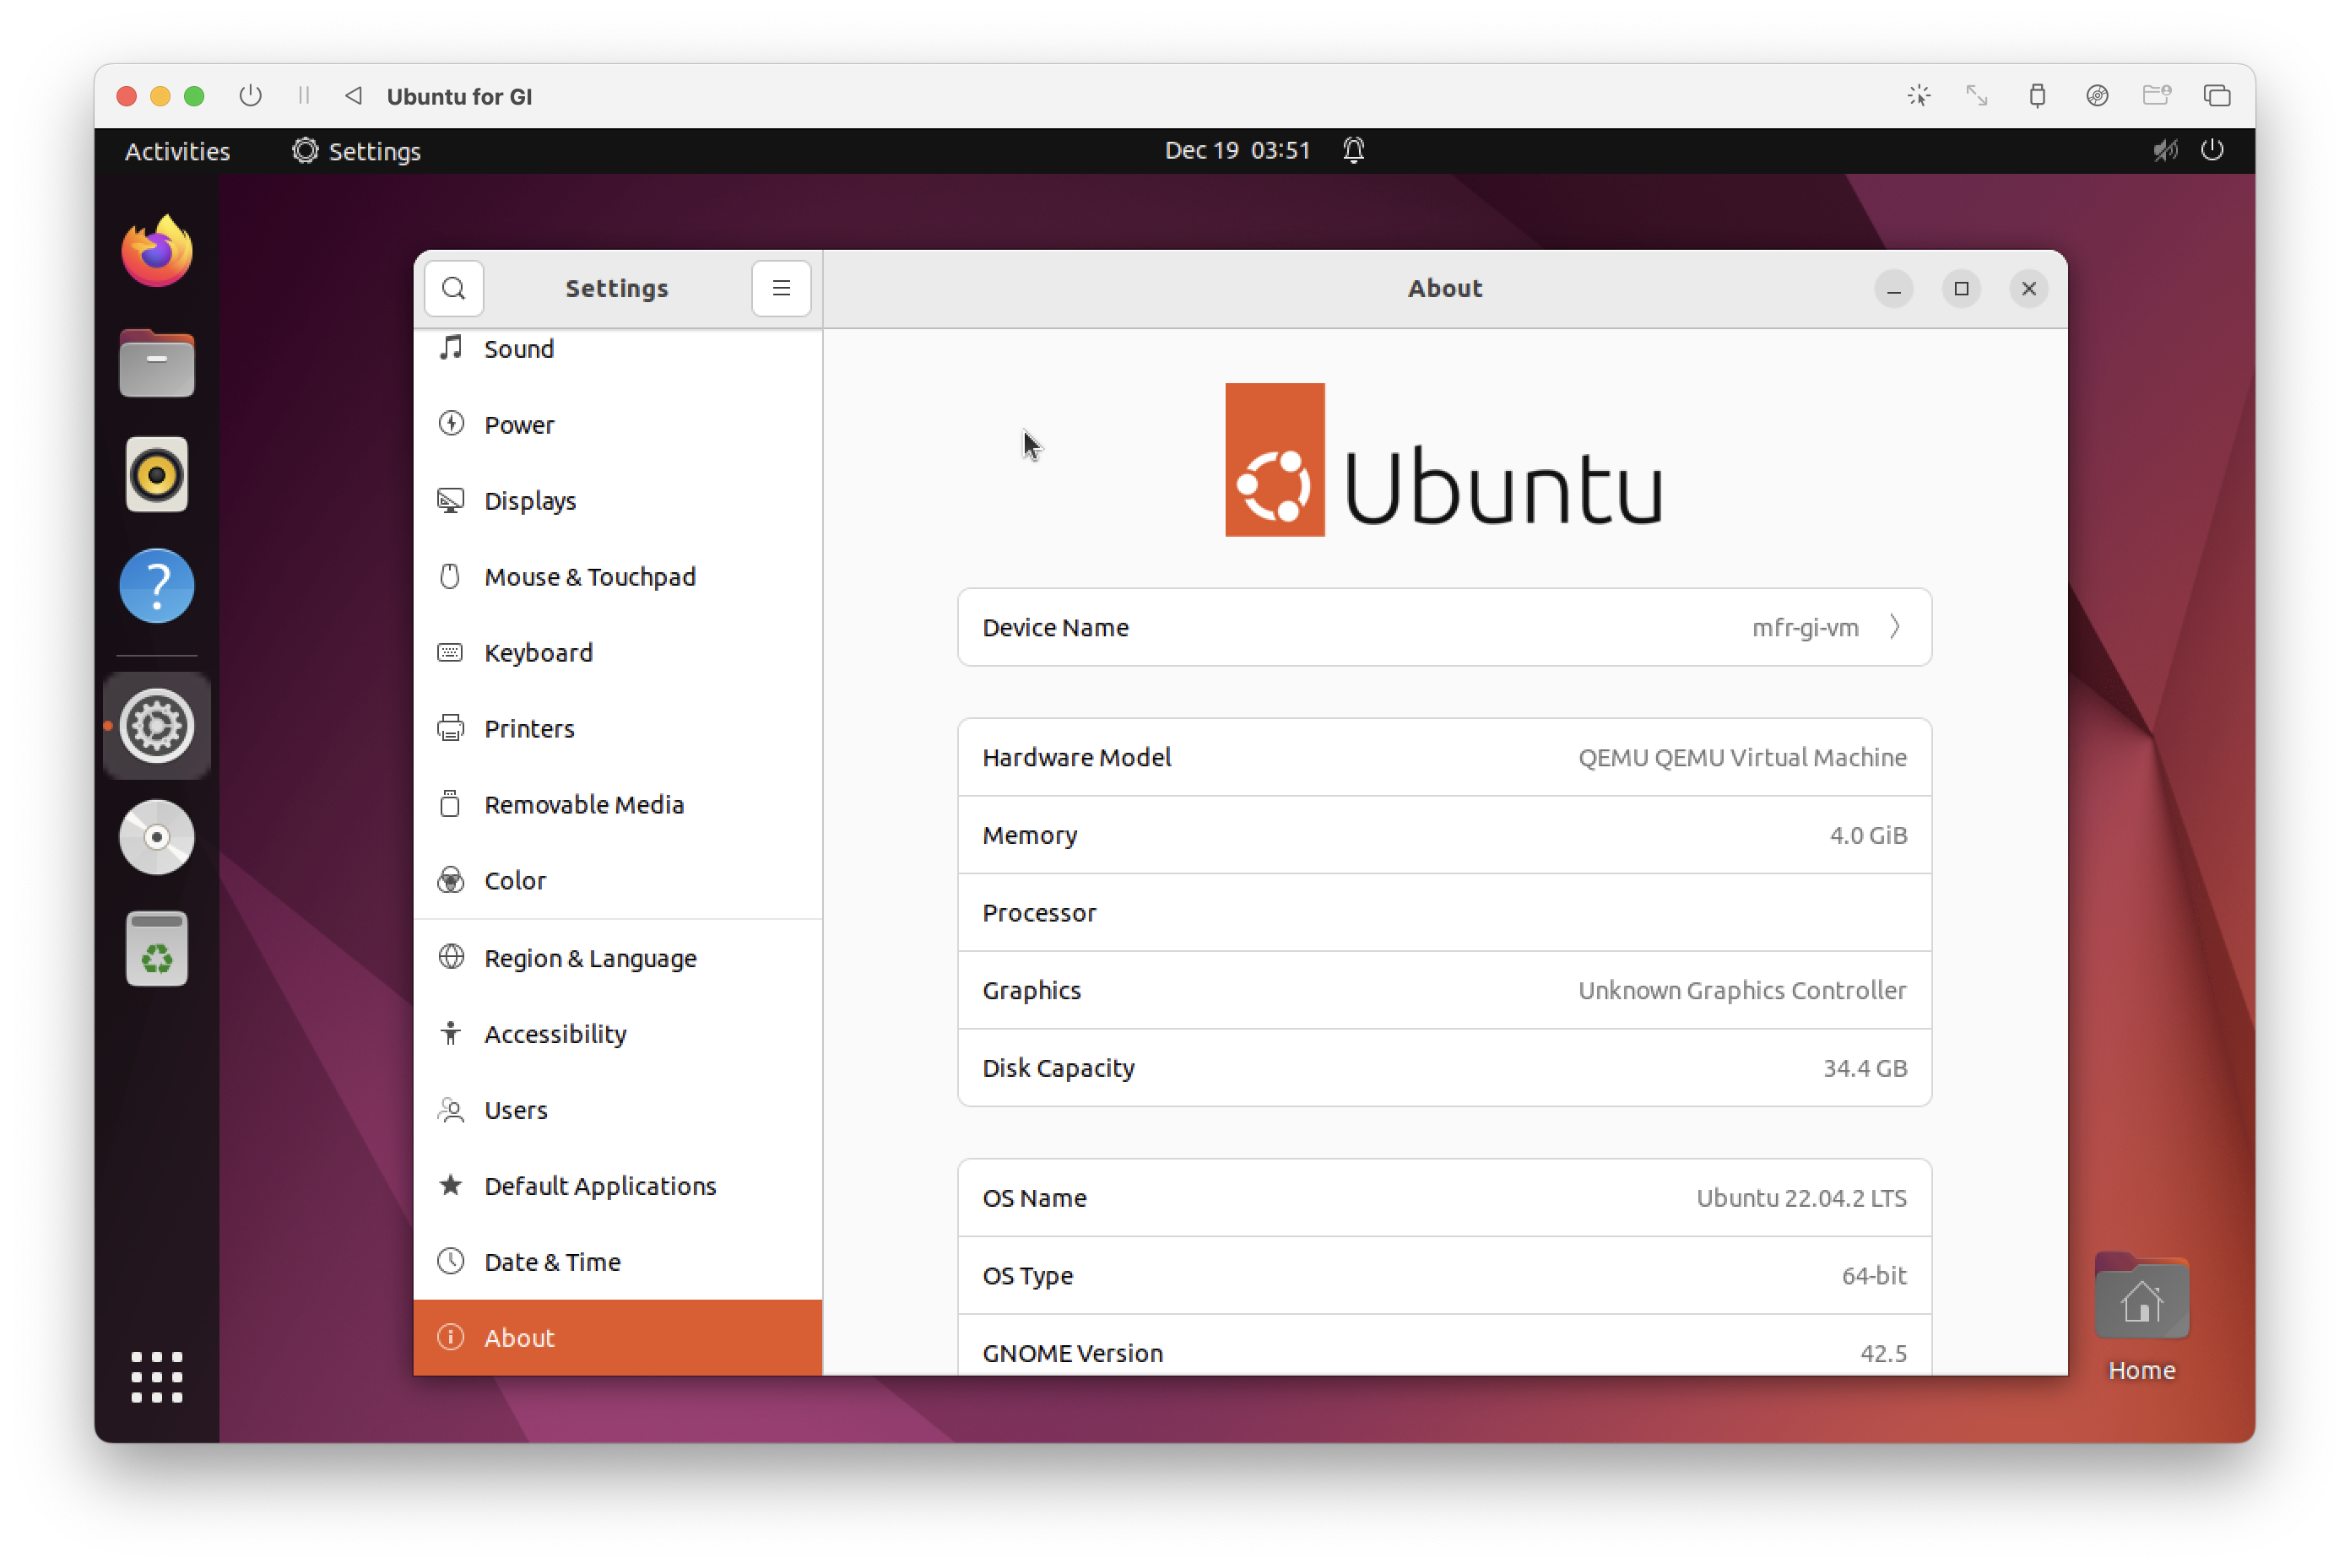
\includegraphics[width=0.75\linewidth]{assets/Screenshot 2023-12-19 at 10.51.04.png}
    \caption{Tangkapan layar \textit{virtual machine} Ubuntu 22.04 (LTS) yang sedang berjalan di perangkat lunak virtualisasi UTM}
    \label{fig:enter-label}
\end{figure}

\subsection{Analisis Sistem Penanganan Notifikasi}

Pengelolaan sistem penanganan notifikasi pada sistem operasi Linux bergantung pada distribusi dan/atau lingkungan desktop (\textit{desktop environment}) yang digunakan, tetapi hampir seluruh implementasi penanganan notifikasi pada sistem operasi Linux berkomunikasi melalui bus perpesanan D-Bus. Sebagai contoh, distribusi Linux yang menggunakan lingkungan \textit{desktop} GNOME menyerahkan pengelolaan notifikasi kepada \textit{desktop} GNOME itu sendiri. Uji coba sistem notifikasi pada Linux dapat dilakukan melalui berbagai cara, seperti
\begin{itemize}
    \item menggunakan perangkat lunak yang normalnya mengirimkan notifikasi (aplikasi \textit{e-mail}, aplikasi perpesanan, dan lain-lain),
    \item mensimulasikan pemanggilan metode (\textit{method}) objek D-Bus khusus yang bertugas menangani notifikasi dengan menggunakan alat (\textit{tool}) pengujian \verb|dbus-send| yang disediakan oleh paket perangkat lunak D-Bus itu sendiri, dan
    \item menggunakan alat (\textit{tool}) \verb|notify-send| yang memiliki fungsi tunggal mengirimkan notifikasi pada \textit{desktop} Linux.
\end{itemize}

Karena kepraktisannya, digunakan alat (\textit{tool}) \verb|notify-send| dalam pengujian awal ini. Alat \verb|notify-send| tersedia secara bawaan pada banyak distribusi Linux seperti Ubuntu dan Fedora. Mengutip halaman manual alat \verb|notify-send| \cite{notify-send-man-page}, alat ini dipanggil dengan bentuk pemanggilan
\begin{lstlisting}[language=bash]
    notify-send [options] {summary} [body]
\end{lstlisting}
dengan dua buah argumen utama:
\begin{itemize}
    \item argumen opsional "\textit{summary}" yang akan tertampil sebagai "judul" notifikasi dan
    \item argumen wajib "\textit{body}" yang berisi konten utama notifikasi dalam bentuk teks.
\end{itemize}
Di samping itu, alat ini juga dapat dipanggil dengan mengikutkan beberapa opsi (\textit{options}) opsional yang berkaitan dengan penampilan notifikasi:
\begin{itemize}
    \item "\verb|-u [tingkat-urgensi]|" atau "\verb|--urgency=[tingkat-urgensi]|" yang menentukan tingkat urgensi notifikasi yang akan ditampilkan (\verb|low|, \verb|normal|, atau \verb|critical|),
    \item "\verb|-t [waktu-kadaluarsa]|" atau "\verb|--expire-time=[waktu-kadaluarsa]|" yang mengatur durasi waktu notifikasi yang tertampil akan menghilang dengan sendirinya (dalam satuan milidetik),
    \item "\verb|-i [lokasi-berkas-ikon]|" atau "\verb|--icon=[lokasi-berkas-ikon]|" yang mengatur ikon yang akan ikut ditampilkan dalam notifikasi,
    \item "\verb|-c [kategori]|" atau "\verb|--category=[kategori]|" yang mengatur kategori notifikasi yang akan tertampil, dan
    \item "\verb|-h [hint]|" atau "\verb|--hint=[hint]|" yang mengatur nilai-nilai \textit{hint} untuk notifikasi yang akan tertampil.
\end{itemize}

Dalam pengujian ini, akan dikirimkan sampel notifikasi sederhana yang hanya memuat judul "Percobaan Notifikasi" dan isi pesan "Halo! Perkenalkan, nama saya Farrel.". Bentuk pemanggilan perintah \verb|notify-send| menjadi seperti berikut.
\begin{lstlisting}[language=bash]
    notify-send "Percobaan Notifikasi" "Halo! Perkenalkan, nama saya Farrel."
\end{lstlisting}
Setelah perintah tersebut dijalankan, muncul notifikasi pada layar komputer seperti pada gambar \ref{ubuntu-notify-send-demo}. Karena Ubuntu (salah satu distribusi Linux) menggunakan lingkungan desktop GNOME, penampilan notifikasi mengikuti gaya penampilan notifikasi pada lingkungan \textit{desktop} GNOME, yaitu di atas layar. Setelah beberapa saat (bergantung pada tingkat urgensi yang telah ditentukan pada pemanggilan perintah \verb|notify-send|), notifikasi akan menghilang dengan sendirinya dan masuk ke panel notifikasi yang disediakan oleh \textit{desktop} GNOME seperti pada gambar \ref{ubuntu-notification-panel}.

\begin{figure}
    \centering
    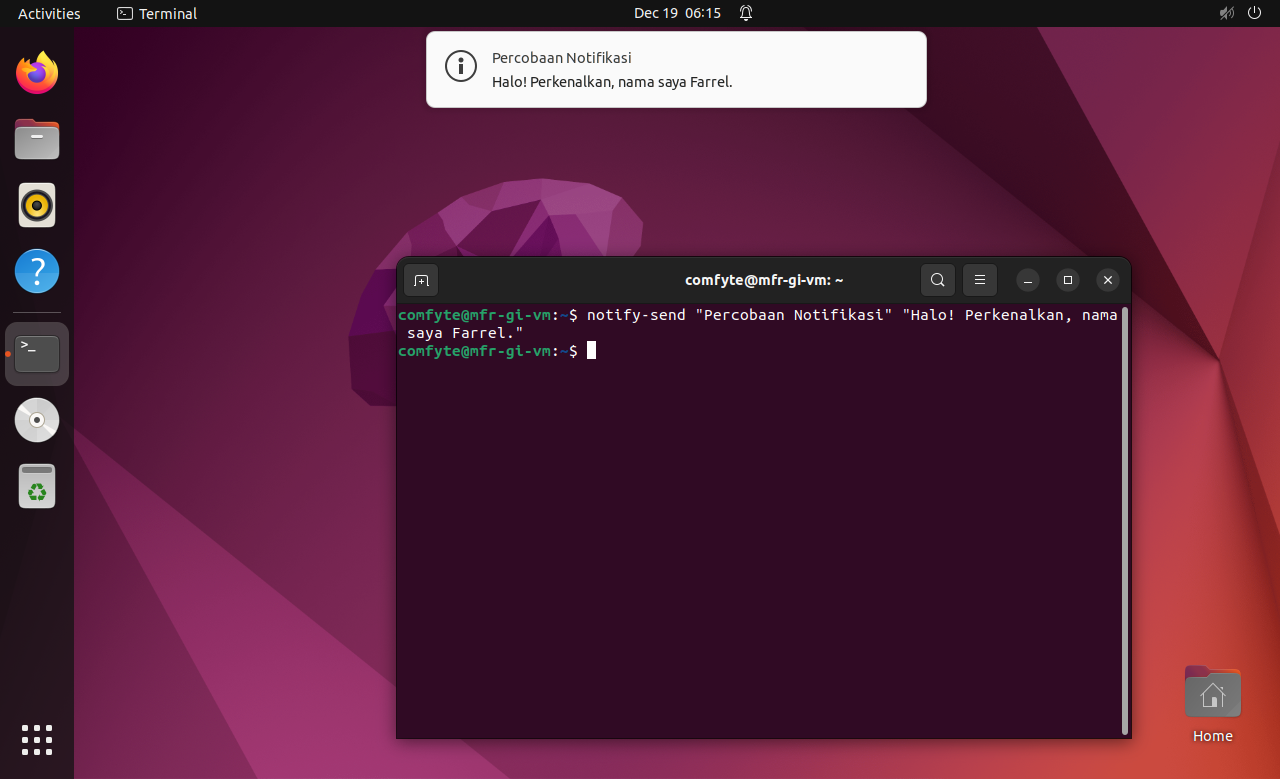
\includegraphics[width=1\linewidth]{assets/Screenshot from 2023-12-19 06-15-10.png}
    \caption{Notifikasi dari notify-send yang berhasil tertampil di \textit{desktop} GNOME di Ubuntu}
    \label{ubuntu-notify-send-demo}
\end{figure}

\begin{figure}
    \centering
    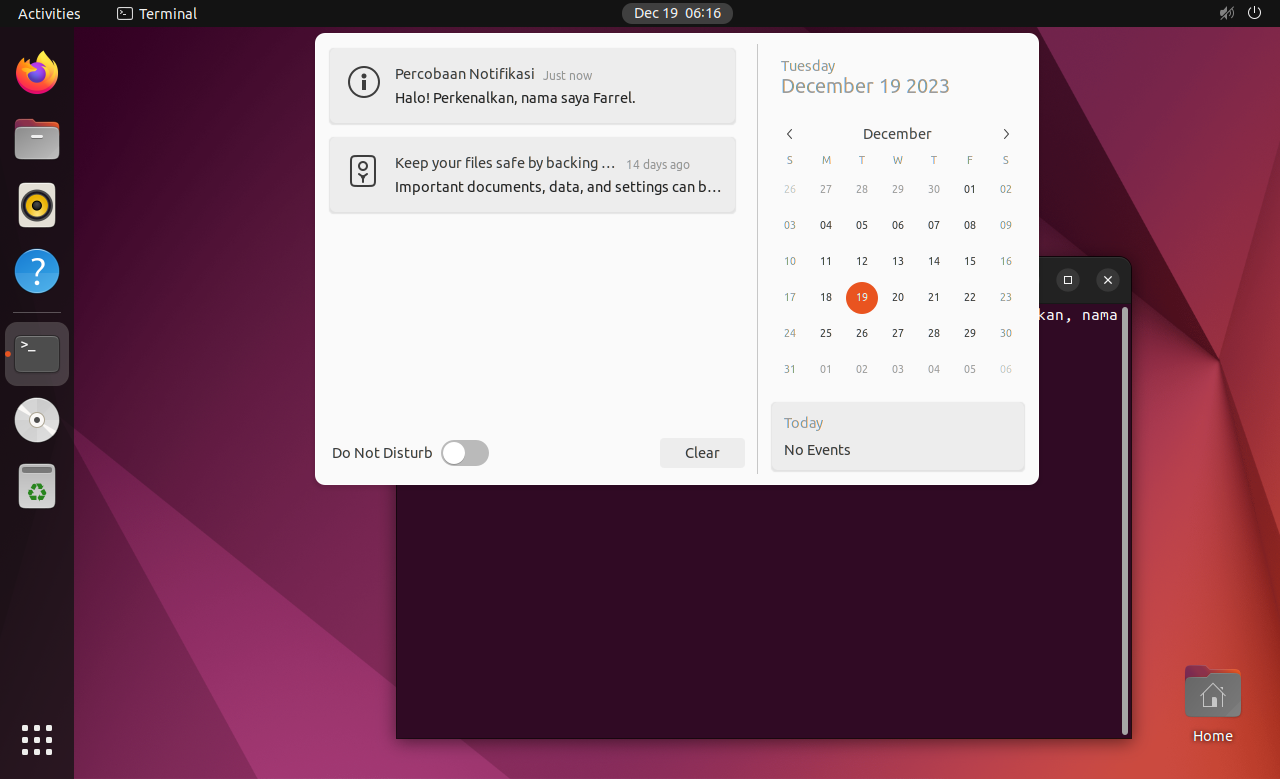
\includegraphics[width=1\linewidth]{assets/Screenshot from 2023-12-19 06-16-29.png}
    \caption{Panel notifikasi di \textit{desktop} GNOME yang mengumpulkan notifikasi-notifikasi lampau yang pernah tertampil}
    \label{ubuntu-notification-panel}
\end{figure}

Pada sistem operasi Linux, dimungkinkan penampilan notifikasi yang lebih kompleks (seperti mengandung tombol-tombol aksi) daripada sekadar notifikasi simpel seperti yang telah diujicobakan. Namun, mengingat alat \verb|notify-send| tidak mendukung jenis notifikasi kompleks seperti itu, pengujian pada bagian ini hanya mengujikan notifikasi yang simpel saja.

\begin{figure}
    \centering
    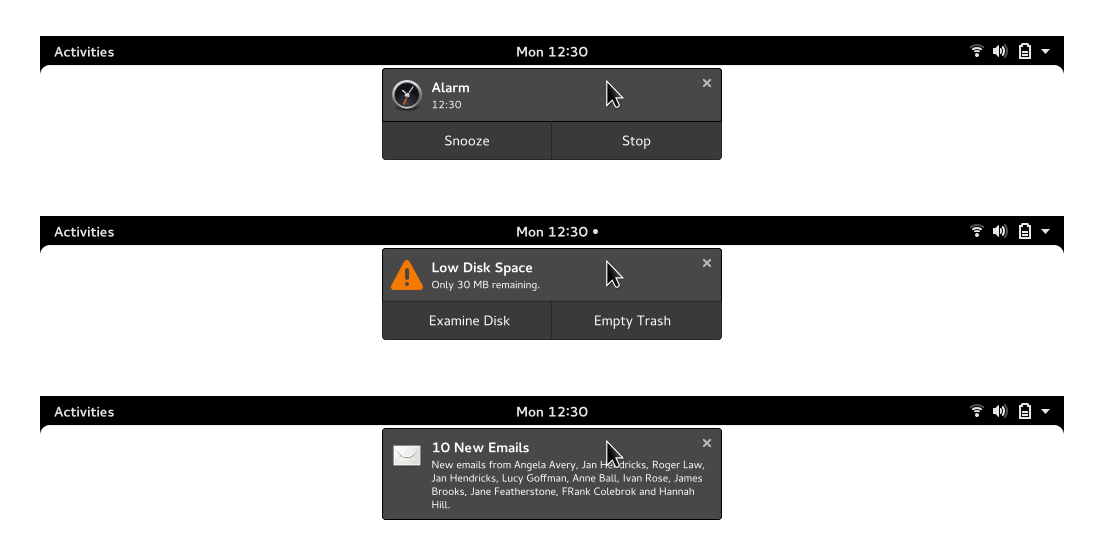
\includegraphics[width=1\linewidth]{assets/banners-expanded.png}
    \caption{Contoh penampilan berbagai jenis notifikasi pada lingkungan \textit{desktop} GNOME \cite{gnome-hig-notifications}; pada \textit{desktop} GNOME, notifikasi kompleks yang memiliki tombol-tombol aksi hanya akan menampilkan tombol-tombol aksi tersebut pada saat notifikasi tersebut berada di bawah kursor \textit{mouse}.}
    \label{example-of-notification-with-action-buttons-on-gnome-desktop}
\end{figure}

Di balik layar, notifikasi yang tertampil tersebut disalurkan dari \verb|notify-send| ke \textit{shell} GNOME melalui bus perpesanan D-Bus yang berjalan pada sesi (\textit{session}) pengguna saat ini. Alat \verb|notify-send| terhubung dengan bus sesi sebagai klien yang memanggil metode \verb|Notify()| pada antarmuka \verb|org.freedesktop.Notifications|; antarmuka tersebut disediakan oleh perangkat lunak \textit{notification server} yang pada lingkungan \textit{desktop} GNOME merupakan \textit{shell} GNOME itu sendiri.

Dalam serangkaian peralatan yang disediakan secara bawaan oleh paket perangkat lunak D-Bus, terdapat alat bernama \verb|dbus-monitor| yang berfungsi memantau detail pesan-pesan yang dipertukarkan di dalam bus perpesanan D-Bus. Secara \textit{default}, penjalanan \verb|dbus-monitor| tanpa memberikan argumen apa pun akan memonitor dan mencetak (di \textit{standard output}) seluruh pesan yang dipertukarkan di bus perpesanan D-Bus sehingga mungkin dirasa berlebihan; penjalanan \verb|dbus-monitor| dapat diatur dengan sebuah argumen berupa perintah filter sehingga pesan-pesan yang dimonitor dan dicetak terbatas pada pesan-pesan yang diinginkan saja. Apabila alat \verb|dbus-monitor| dijalankan dengan perintah lengkap
\begin{lstlisting}[language=bash]
    dbus-monitor "path='/org/freedesktop/Notifications'"
\end{lstlisting}
untuk memulai proses pemantauan dan perintah pengiriman notifikasi yang menggunakan \verb|notify-send| di atas dijalankan ulang, jendela terminal tempat penjalanan \verb|dbus-monitor| akan mengeluarkan informasi seperti berikut.
\begin{lstlisting}
method call time=1702972516.257275 sender=:1.48 -> destination=:1.35 serial=31 path=/org/freedesktop/Notifications; interface=org.freedesktop.Notifications; member=Notify
   string "notify-send"
   uint32 0
   string ""
   string "Percobaan Notifikasi"
   string "Halo! Perkenalkan, nama saya Farrel."
   array [
   ]
   array [
      dict entry(
         string "urgency"
         variant             byte 1
      )
      dict entry(
         string "sender-pid"
         variant             uint32 3347
      )
   ]
   int32 -1
\end{lstlisting}

Keluaran (\textit{output}) penjalanan perintah \verb|dbus-monitor| secara gamblang menunjukkan informasi-informasi teknis pada suatu penampilan notifikasi di \textit{desktop} Linux. Di samping dokumen spesifikasi resmi penanganan notifikasi di Linux sebagai acuan utama \cite{xdg-desktop-notifications-specification}, hasil keluaran alat-alat seperti \verb|dbus-monitor| dapat sangat bermanfaat untuk menginspeksi dan men-\textit{debug} mekanisme penanganan notifikasi pada tahap-tahap pengembangan yang dilakukan selanjutnya.

\subsection{Analisis Sistem Kontrol Media}

Sistem-sistem operasi modern menawarkan antarmuka pengontrolan yang mudah (umumnya berbentuk panel) saat pengguna memulai pemutaran media, baik musik, video, maupun jenis media lainnya; sistem operasi Linux pun tidak berbeda. Sistem operasi Linux menawarkan akses cepat dan universal untuk mengontrol media yang sedang diputar oleh aplikasi-aplikasi pemutar media dengan peletakan spesifik \textit{user interface} yang menyesuaikan lingkungan \textit{desktop} yang digunakan, tetapi dengan protokol dan antarmuka yang seragam antarimplementasi tersebut. Protokol dan antarmuka yang dimaksud bernama Media Player Remote Interfacing Specification (MPRIS).

Serupa dengan sistem penanganan notifikasi pada sistem operasi Linux, sistem pengontrolan media pada sistem operasi Linux juga memanfaatkan bus perpesanan D-Bus yang berjalan pada sesi pengguna (\textit{user session}) yang aktif. Namun, sebagai sesama klien D-Bus, sistem pengontrolan media ini bertindak berbeda dengan sistem penanganan media yang telah dijelaskan pada bagian sebelumnya; bagian ini akan mengeksplor sistem pengontrolan media pada Linux (MPRIS) secara lebih mendetail serta perbedaan dengan sistem penanganan notifikasi tersebut.

Apabila pengguna sistem operasi Linux memutar media (musik, video, atau lainnya) di suatu perangkat lunak pemutar media yang mendukung, perangkat lunak tersebut akan mengekspor informasi dan data mengenai pemutaran media tersebut ke bagian \textit{shell} sistem operasi yang bertugas menangani penampilan kontrol media (untuk contoh pada Ubuntu, lihat gambar \ref{ubuntu-media-controls}. Penyaluran informasi dan data ini dilakukan melalui bus perpesanan D-Bus yang berjalan di sesi pengguna \textit{user session} yang bersangkutan.

\begin{figure}
    \centering
    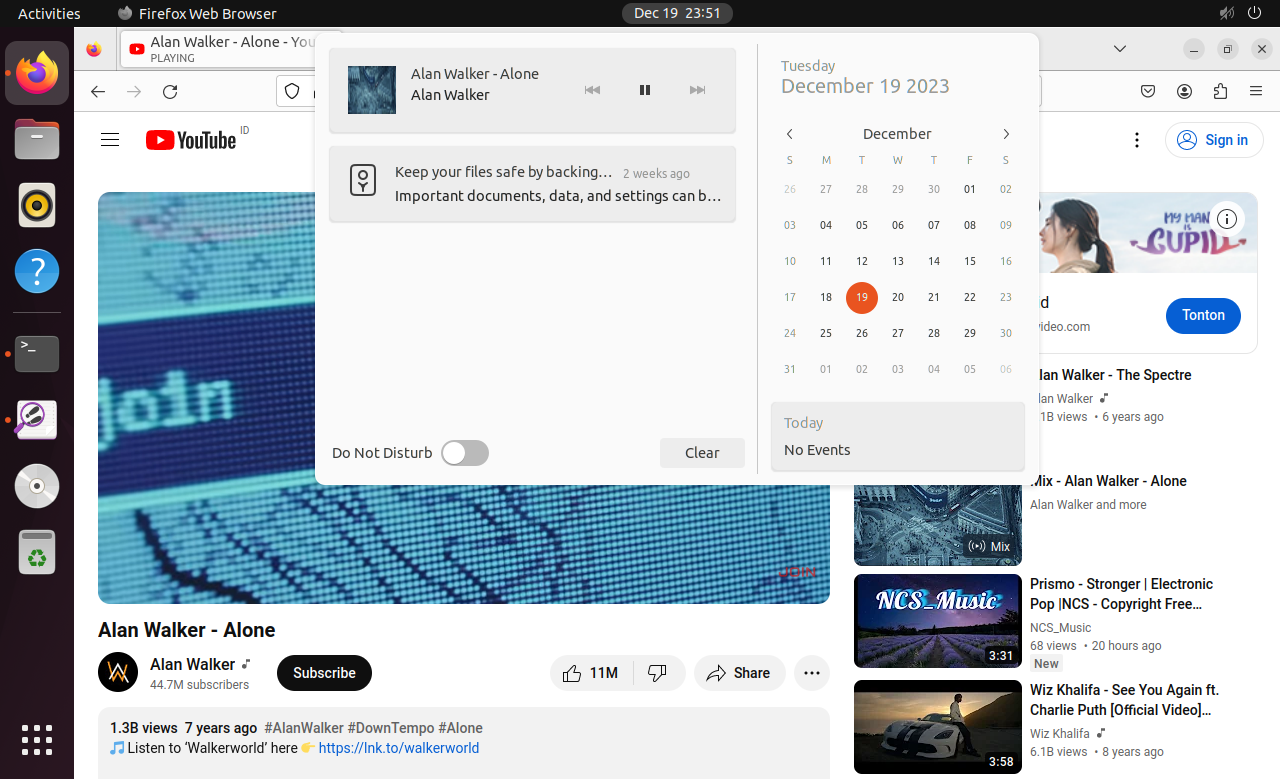
\includegraphics[width=1\linewidth]{assets/Screenshot from 2023-12-19 23-51-47.png}
    \caption{Contoh kontrol media yang muncul di antarmuka pengguna (\textit{graphical user interface}) \textit{shell} Ubuntu saat pengguna mulai memutar video YouTube}
    \label{ubuntu-media-controls}
\end{figure}

Penggunaan alat \verb|dbus-monitor| yang terfilter pada pemonitoran \textit{path} tempat pengomunikasian pemutaran media MPRIS, \path{/org/mpris/MediaPlayer2}, menunjukkan informasi dan data yang berkaitan dengan media yang sedang diputar beserta statusnya.
\begin{lstlisting}
signal time=1703030006.305799 sender=:1.179 -> destination=(null destination) serial=24 path=/org/mpris/MediaPlayer2; interface=org.freedesktop.DBus.Properties; member=PropertiesChanged
   string "org.mpris.MediaPlayer2.Player"
   array [
      dict entry(
         string "Metadata"
         variant             array [
               dict entry(
                  string "mpris:trackid"
                  variant                      object path "/org/mpris/MediaPlayer2/firefox"
               )
               dict entry(
                  string "xesam:title"
                  variant                      string "Marshmello - Alone (Official Music Video)"
               )
               dict entry(
                  string "xesam:album"
                  variant                      string ""
               )
               dict entry(
                  string "xesam:artist"
                  variant                      array [
                        string "Marshmello"
                     ]
               )
            ]
      )
   ]
   array [
   ]
signal time=1703030006.312580 sender=:1.179 -> destination=(null destination) serial=25 path=/org/mpris/MediaPlayer2; interface=org.freedesktop.DBus.Properties; member=PropertiesChanged
   string "org.mpris.MediaPlayer2.Player"
   array [
      dict entry(
         string "PlaybackStatus"
         variant             string "Playing"
      )
   ]
   array [
   ]
\end{lstlisting}

Berdasarkan hasil keluaran perintah \verb|dbus-monitor|, dapat terlihat bahwa tipe pesan yang disampaikan adalah sinyal (\textit{signal}) yang menandakan bahwa pengomunikasian MPRIS tidak menggunakan pemanggilan metode (\textit{method}) seperti pada sistem penanganan notifikasi. Hal ini juga didukung oleh dokumen spesifikasi resmi yang memaparkan bagaimana protokol dan antarmuka MPRIS bekerja \cite{xdg-mpris-specification}. Alih-alih menggunakan pemanggilan metode (\textit{method}), MPRIS memanfaatkan elemen properti (\textit{property}) yang dimiliki oleh objek \path{/org/mpris/MediaPlayer2} untuk menyimpan informasi dan data tentang media yang sedang diputar dan bergantung pada sinyal \verb|PropertiesChanged| pada antarmuka standar \verb|org.freedesktop.DBus.Properties| untuk mengomunikasikan perubahannya kepada klien-klien lain yang berkepentingan seperti lingkungan desktop Linux yang bertugas menampilkan pemutaran media tersebut.

Hal menarik terjadi apabila pengguna memutar media pada dua atau lebih perangkat lunak pemutaran media (meskipun tidak secara bersamaan dalam satu waktu). Dalam hal ini, lingkungan \textit{desktop} Linux (GNOME pada contoh ini) menampilkan semua media yang sedang diputar tersebut (lihat gambar \ref{ubuntu-multiple-media-playbacks}. Menurut pengamatan awal penulis, terdapat dua jenis informasi di balik layar yang dapat memungkinkan hal ini:
\begin{itemize}
    \item Nilai \verb|mpris:trackid| pada properti "Metadata" yang terlihat mengemban informasi unik mengenai media yang sedang diputar dan/atau
    \item Sinyal \verb|NameOwnerChanged| pada antarmuka \verb|org.freedesktop.DBus| yang mengomunikasikan apabila suatu perangkat lunak atau aplikasi dibuka atau ditutup yang mengakibatkan munculnya atau hilangnya klien yang bersangkutan pada bus perpesanan D-Bus.
\end{itemize}

\begin{figure}
    \centering
    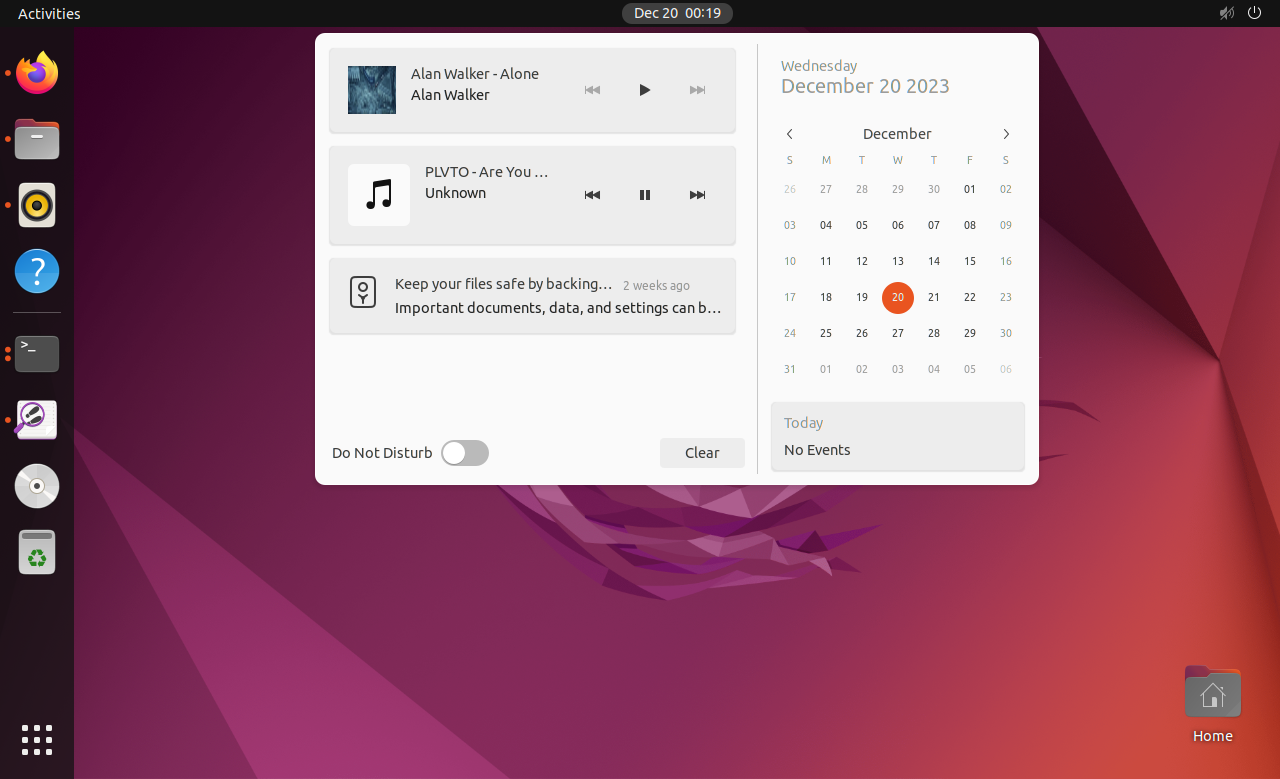
\includegraphics[width=1\linewidth]{assets/Screenshot from 2023-12-20 00-19-07.png}
    \caption{Pemutaran media pada dua aplikasi, Firefox (pemutaran di situs web YouTube) dan Rhythmbox (aplikasi pemutar berkas musik lokal), di Ubuntu menyebabkan \textit{shell} GNOME pada Ubuntu menampilkan semua media yang sedang diputar tersebut.}
    \label{ubuntu-multiple-media-playbacks}
\end{figure}

\section{Analisis Ekosistem pada Masing-Masing Platform (Linux dan Windows)}

Guna memungkinkan proses \textit{bridging} lingkungan WSL dengan lingkungan \textit{host} Windows dalam aspek penanganan notifikasi dan aspek kontrol media, diperlukan analisis mendalam mengenai antarmuka teknis yang membawahi kedua aspek tersebut.

\subsection{Analisis Sistem Penanganan Notifikasi}

Sistem operasi Linux memiliki standar penyampaian notifikasi bernama FreeDesktop Desktop Notifications Specification \cite{xdg-desktop-notifications-specification}. Spesifikasi ini mengatur mekanisme penyampaian notifikasi antarklien D-Bus dengan menetapkan antarmuka standar yang harus disetujui oleh klien-klien yang akan berpartisipasi, yakni \verb|org.freedesktop.Notifications| yang terletak pada objek \path{/org/freedesktop/Notifications}. Antarmuka tersebut mengandung metode "Notify()" yang bertugas mengirimkan notifikasi dan memiliki sejumlah parameter yang perlu menjadi perhatian dalam pengerjaan tugas akhir ini. Sebagian besar parameter pada antarmuka ini bersifat opsional kecuali properti \textit{body} konten yang bersifat wajib dicantumkan oleh perangkat lunak atau aplikasi pengirim notifikasi.
\begin{itemize}
    \item \textbf{Parameter nama aplikasi (app\_name)}\\
    Parameter ini berisi informasi nama perangkat lunak atau aplikasi yang mengirimkan notifikasi.
    
    \item \textbf{Parameter "replaces ID" (replaces\_id)}\\
    Parameter ini berisi informasi identitas (ID) notifikasi lain yang telah tertampil untuk digantikan oleh notifikasi yang sedang dikirimkan saat ini.

    \item \textbf{Parameter ikon notifikasi (app\_icon)}\\
    Parameter ini mengatur ikon yang ikut tertampil di notifikasi yang dikirimkan. Parameter ini berisi lokasi berkas ikon di dalam \textit{file system}.

    \item \textbf{Parameter ringkasan konten (summary)}\\
    Parameter ini berisi ringkasan singkat (\textit{summary}) notifikasi yang akan ditampilkan dengan peletakan dan penampilan teks yang lebih prominen dibandingkan dengan teks konten yang lain. Parameter ini dapat dikatakan pula sebagai "judul" notifikasi tersebut.
    
    \item \textbf{Parameter \textit{body} konten (body)}\\
    Parameter ini berisi konten utama notifikasi dalam bentuk teks.
    
    \item \textbf{Parameter aksi (actions)}\\
    Parameter ini menentukan aksi-aksi (\textit{actions}) yang dapat muncul pada notifikasi yang tertampil seperti tombol.
    
    \item \textbf{Parameter \textit{hints} (hints)}\\
    Parameter ini digunakan oleh perangkat lunak atau aplikasi pengirim notifikasi untuk memberi informasi lebih yang bersifat lain-lain kepada \textit{notification server}.
    
    \item \textbf{Parameter durasi waktu kadaluarsa (expire\_timeout)}\\
    Parameter ini mengatur durasi lamanya suatu notifikasi (dalam milidetik) akan terhapus dengan sendirinya. Parameter ini juga dapat diatur dengan nilai \verb|-1| untuk menyerahkan pengelolaan waktu tertampil notifikasi yang bersangkutan kepada \textit{notification server} atau nilai \verb|0| agar notifikasi tidak pernah terhapus dengan sendirinya.
\end{itemize}

Elemen-elemen di atas diatur dalam suatu pengiriman notifikasi sebagai argumen-argumen pemanggilan metode "Notify()" pada antarmuka \path{org.freedesktop.Notifications}. Dengan kata lain, metode "Notify()" ini memiliki \textit{method signature} sebagai berikut.
\begin{lstlisting}
/* Tipe return-nya adalah UINT32 */
org.freedesktop.Notifications.Notify(STRING app_name,
                                     UINT32 replaces_id,
                                     STRING app_icon,
                                     STRING summary,
                                     STRING body,
                                     ARRAY actions,
                                     ARRAY hints,
                                     INT32 expire_timeout);
\end{lstlisting}

Di sisi Windows, terdapat berbagai jenis solusi penampilan notifikasi yang disediakan yang bergantung pada jenis \textit{toolkit} pemrograman GUI yang digunakan (Universal Windows Platform atau Windows Runtime, Windows Presentation Foundation, Windows Forms, atau jenis \textit{toolkit} lainnya). Salah satu solusi penampilan notifikasi di Windows dan solusi yang digunakan dalam tugas akhir ini adalah ToastNotification yang disediakan oleh platform bawaan Windows Runtime (WinRT) dan umumnya digunakan oleh aplikasi-aplikasi Windows berbasis \textit{toolkit} Universal Windows Platform (UWP) \cite{microsoft-toast-notification-overview}. Notifikasi pada ToastNotification umumnya dikirimkan dalam format XML dengan \textit{schema} (struktur dokumen) yang telah ditetapkan. \textit{Schema} tersebut mengatur parameter-parameter yang dapat diatur dalam menampilkan notifikasi. Mengutip situs web dokumentasi Microsoft pada bagian pendefinisian \textit{schema} ToastNotification \cite{microsoft-toast-notification-schema}, berikut beberapa di antara elemen-elemen yang tersedia untuk diatur pada struktur XML notifikasi yang ingin ditampilkan.

\begin{itemize}
    \item \textbf{Elemen "<binding>"}\\
    Elemen ini digunakan untuk menentukan templat notifikasi \textit{toast} yang akan ditampilkan.
    
    \item \textbf{Elemen "<text>"}\\
    Elemen ini digunakan untuk mengatur teks yang muncul pada notifikasi \textit{toast}.
    
    \item \textbf{Elemen "<toast>"}\\
    Elemen ini merupakan elemen \textit{parent} tunggal yang mencakup seluruh elemen-elemen lain pada notifikasi \textit{toast}.
    
    \item \textbf{Elemen "<visual>"}\\
    Elemen ini digunakan untuk mengandung satu buah elemen \verb|<binding>| yang telah dijelaskan pada poin pertama.
\end{itemize}

Menganalisis kedua ekosistem penampilan notifikasi tersebut, ekuivalensi dan penghubungan keduanya dapat dilakukan dengan mengacu pada tabel \ref{}.

\begin{table}[h]
    \centering
    \caption{Tabel ekuivalensi elemen-elemen notifikasi di Linux (WSL) dengan Windows}
    \begin{tabularx}{\textwidth}{|c|p{3cm}|X|X|} \hline
        \textbf{No.} & \textbf{Elemen} & \textbf{Mekanisme di Linux (WSL)} & \textbf{Metode penghubungan dengan Windows}\\ \hline
        1 & Nama aplikasi pengirim notifikasi & Parameter "app\_name" & Mengatur bagian konten elemen \verb|<text>|\\ \hline
        2 & Judul/ringkasan notifikasi & Parameter "summary" & Memasukkan ke baris pertama di konten elemen \verb|<text>| dan mengatur baris pertama tersebut agar tercetak tebal (\textit{bold})\\ \hline
        3 & Konten utama (\textit{body}) notifikasi & Parameter "body" & Memasukkan ke baris-baris nonjudul di konten elemen \verb|<text>|\\ \hline
    \end{tabularx}
    \label{wsl-and-windows-notification-system-equivalence-table}
\end{table}

\subsection{Analisis Sistem Kontrol Media}

Sistem operasi Linux memiliki standar sistem pengontrolan media universal bernama Media Plyer Remote Interfacing Specification (MPRIS) \cite{xdg-mpris-specification}. Spesifikasi ini mengatur mekanisme komunikasi dalam D-Bus untuk pengontrolan media dengan menetapkan sejumlah antarmuka standar yang harus disetujui oleh klien-klien yang akan berpartisipasi, yakni antarmuka \verb|org.mpris.MediaPlayer2| dan antarmuka \verb|org.mpris.MediaPlayer2.Player| yang kedua terletak pada objek \path{/org/mpris/MediaPlayer2}. Berikut elemen-elemen dalam antarmuka tersebut, baik properti maupun metode, yang perlu diperhatikan dalam pengerjaan tugas akhir ini.

\begin{itemize}
    \item Properti "PlaybackStatus" pada antarmuka \verb|org.mpris.MediaPlayer2.Player| yang mengindikasikan status pemutaran media ("Playing", "Paused", atau "Stopped").

    \item Properti "Metadata" pada antarmuka \verb|org.mpris.MediaPlayer2.Player| berisi informasi-informasi tentang media yang sedang diputar, seperti judul media (\verb|xesam:title|), artis (\verb|xesam:artist|), dan artis album (\verb|xesam:albumArtist|), dalam bentuk \textit{array} yang berisi pasangan nama-nilai (\textit{key-value pairs}).
    
    \item Properti "CanGoNext" pada antarmuka \verb|org.mpris.MediaPlayer2.Player| yang mengindikasikan apakah perangkat lunak yang sedang memutar media saat ini memungkinkan pemindahan pemutaran ke media selanjutnya.
    
    \item Properti "CanGoPrevious" pada antarmuka \verb|org.mpris.MediaPlayer2.Player| yang mengindikasikan apakah perangkat lunak yang sedang memutar media saat ini memungkinkan pemindahan pemutaran ke media sebelumnya.
    
    \item Properti "CanPlay" pada antarmuka \verb|org.mpris.MediaPlayer2.Player| yang mengindikasikan apakah perangkat lunak pemutar media saat ini dapat memulai pemutaran media (\textit{play}).
    
    \item Properti "CanPause" pada antarmuka \verb|org.mpris.MediaPlayer2.Player| yang mengindikaskan apakah perangkat lunak pemutar media saat ini dapat menjeda pemutaran media saat ini (\textit{pause}).
    
    \item Metode "Next()" pada antarmuka \verb|org.mpris.MediaPlayer2.Player| yang memerintahkan klien yang sedang memutar media untuk berpindah ke media selanjutnya apabila properti "CanGoNext" bernilai benar (\textit{true}).
    
    \item Metode "Previous()" pada antarmuka \verb|org.mpris.MediaPlayer2.Player| yang memerintahkan klien yang sedang memutar media untuk berpindah ke media sebelumnya apabila properti "CanGoPrevious" bernilai benar (\textit{true}).
    
    \item Metode "PlayPause()" pada antarmuka \verb|org.mpris.MediaPlayer2.Player| yang memerintahkan klien yang sedang memutar media untuk menjeda media apabila sedang memutar media (jika properti "CanPause" bernilai benar (\textit{true})) atau memulai pemutaran media apabila media sedang dijeda (jika properti "CanPlay" bernilai benar (\textit{true})).
    
    \item Metode "Play()" pada antarmuka \verb|org.mpris.MediaPlayer2.Player| yang memerintahkan klien yang sedang memutar media untuk menjeda media yang sedang memutar diputar apabila properti "CanPlay" bernilai benar (\textit{true}).
    
    \item Metode "Stop()" pada antarmuka \verb|org.mpris.MediaPlayer2.Player| yang memerintahkan klien yang sedang memutar media untuk menghentikan media yang sedang diputar.
\end{itemize}

Seperti yang telah dijelaskan di atas, antarmuka \verb|org.mpris.MediaPlayer2.Player| memiliki properti dan metode. Apabila klien-klien lain dalam bus perpesanan D-Bus yang sama ingin memantau perubahan pada properti-properti tersebut, klien-klien tersebut dapat menunggu sinyal \verb|PropertiesChanged| yang dikeluarkan oleh antarmuka \verb|org.freedesktop.DBus| pada objek \path{/org/mpris/MediaPlayer2}.

Di sisi Windows, sistem kontrol media pada pemutaran media oleh perangkat-perangkat lunak 
dikomunikasikan melalui standar System Media Transport Controls (SMTC) yang mengatur sejumlah mekanisme yang wajib dipatuhi dan dilakukan oleh perangkat-perangkat lunak di Windows yang ingin berpartisipasi \cite{microsoft-docs-manual-control-of-the-smtc}. Berikut elemen-elemen yang digunakan untuk mengatur penampilan kontrol media di \textit{shell} Windows yang penting diperhatikan dalam pengerjaan tugas akhir ini.
\begin{itemize}
    \item Properti \verb|IsPlayEnabled| pada \textit{instance} objek SystemMediaTransportControls yang dapat diatur (\textit{settable}) dengan nilai \textit{boolean} benar atau salah.
    
    \item Properti \verb|IsPauseEnabled| pada \textit{instance} objek SystemMediaTransportControls yang dapat diatur (\textit{settable}) dengan nilai \textit{boolean} benar atau salah.
    
    \item Properti \verb|PlaybackStatus| pada \textit{instance} objek SystemMediaTransportControls yang dapat diatur (\textit{settable}) dengan status pemutaran media saat ini (berputar, terjeda, terhenti, atau tertutup) yang terletak di objek enumerasi (\verb|enum|) MediaPlaybackStatus.
    
    \item Properti \verb|Type| di dalam properti \path{DisplayUpdater} pada \textit{instance} objek SystemMediaTransportControls yang dapat diatur (\textit{settable}) dengan tipe media yang sedang diputar saat ini menggunakan nilai-nilai yang berada di dalam objek enumerasi (\verb|enum|) MediaPlaybackType (\verb|Music|, \verb|Video|, \verb|Image|, atau \verb|Unknown|).
    
    \item Properti \verb|Artist| di dalam rantai properti \path{DisplayUpdater.MusicProperties} pada \textit{instance} objek SystemMediaTransportControls yang dapat diatur (\textit{settable}) dengan teks berisi informasi nama-nama artis/penyanyi pada media yang sedang diputar.
    
    \item Properti \verb|AlbumArtist| di dalam rantai properti \path{DisplayUpdater.MusicProperties} pada \textit{instance} objek SystemMediaTransportControls yang dapat diatur (\textit{settable}) dengan teks berisi informasi nama-nama artis album pada media yang sedang diputar.
    
    \item Properti \verb|Title| di dalam rantai properti \path{DisplayUpdater.MusicProperties} pada \textit{instance} objek SystemMediaTransportControls yang dapat diatur dengan teks berisi informasi judul media yang sedang diputar.

\end{itemize}

Berdasarkan kedua ekosistem pemutaran media (\textit{Linux dan Windows}) yang telah dijabarkan di atas, dapat dilakukan proses ekuivalensi dan mekanisme penghubungan keduanya seperti pada \autoref{wsl-and-windows-media-control-equivalence-table}.

\begin{table}[h]
    \centering
    \caption{Tabel ekuivalensi elemen-elemen pengontrolan media di Linux (WSL) dengan Windows}
    \begin{tabularx}{\textwidth}{|c|p{3cm}|X|X|} \hline
        \textbf{No.} & \textbf{Elemen} & \textbf{Mekanisme di Linux (WSL)} & \textbf{Metode penghubungan dengan Windows}\\ \hline
        1 & Status pemutaran media & Properti "PlaybackStatus" & Mengatur properti \verb|PlaybackStatus|\\ \hline
        2 & Dukungan pemulaian pemutaran media (\textit{play}) & Properti "CanPlay" & Mengatur properti \verb|IsPlayEnabled|\\ \hline
        3 & Dukungan penjedaan pemutaran media (\textit{pause}) & properti "CanPause" & Mengatur properti \verb|IsPauseEnabled|\\ \hline
        4 & Judul media & Nilai \verb|xesam:title| pada properti "Metadata" & Mengatur Properti \path{DisplayUpdater.MusicProperties.Title}\\ \hline
        5 & Album media & Nilai \verb|xesam:album| pada properti "Metadata" & Mengatur properti \path{DisplayUpdater.MusicProperties.Album}\\ \hline
        6 & Artis media & Nilai \verb|xesam:artist| pada properti "Metadata" & Mengatur properti \path{DisplayUpdater.MusicProperties.Artist}\\ \hline
        7 & Album artis media & Nilai \verb|xesam:albumArtist| pada properti "Metadata" & Mengatur properti \path{DisplayUpdater.MusicProperties.AlbumArtist}\\ \hline
    \end{tabularx}
    \label{wsl-and-windows-media-control-equivalence-table}
\end{table}

\section{Pengembangan Perangkat Lunak FancyWSL}

Guna mencapai tujuan utama tugas akhir ini, dikembangkan sebuah perangkat lunak bernama "FancyWSL" yang bertugas menjembatani aspek penanganan notifikasi dan aspek kontrol media pada lingkungan Windows Subsystem for Linux (WSL) dengan lingkungan \textit{host} Windows. Seluruh kode sumber yang dikembangkan dalam tugas akhir ini juga tersedia untuk diakses oleh publik di platform GitHub di alamat \href{https://github.com/comfyte/skripsi}{https://github.com/comfyte/skripsi}, tepatnya di direktori \path{FancyWSL/}. Perangkat lunak ini dikembangkan dengan menggunakan bahasa pemrograman Python dan sejumlah pustaka pemrograman (\textit{library}) pihak ketiga dengan pertimbangan yang telah dibahas pada Bab II. Secara garis besar, proyek perangkat lunak ini dikembangkan dengan struktur direktori yang mengacu sepatuh mungkin kepada konvensi penstrukturan direktori dan penamaan berkas proyek Python pada umumnya. Struktur direktori yang dimaksud berikut penjelasan singkatnya adalah sebagai berikut.

\begin{verbatim}
fwsl_daemon/
├── __main__.py
├── helpers/
│   ├── __init__.py
│   └── verify_platform.py
├── services/
│   ├── __init__.py
│   ├── media_control.py
│   └── notifications.py
└── shell/
    ├── __init__.py
    ├── persistent_tray_icon.py
    ├── smtc.py
    └── toast_notification.py
\end{verbatim}

\begin{itemize}
    \item Berkas \verb|__main__.py| merupakan berkas utama yang bertindak sebagai \textit{entry point} penjalanan perangkat lunak FancyWSL.

    \item Direktori \verb|helpers| mengandung modul-modul kode yang bersifat umum dan dapat digunakan di berbagai berkas kode program.

    \item Direktori \verb|services| mengandung modul-modul yang menangani fungsi pengantarmukaan (\textit{interfacing}) dengan bus perpesanan D-Bus di WSL yang saat ini telah dapat diakses di Windows melalui TCP.

    \item Direktori \verb|shell| mengandung modul-modul yang berfungsi mengintegrasikan perangkat lunak FancyWSL dengan beragam aspek \textit{shell} Windows, yaitu aspek penampilan notifikasi dan aspek kontrol media.

    \item Berkas \verb|__init__.py| pada masing-masing direktori berfungsi menandakan bahwa direktori-direktori tersebut bisa diimpor (\textit{importable}) sebagai satu kesatuan modul \cite{oliphant2007python}.
\end{itemize}

Pengembangan perangkat lunak FancyWSL melibatkan sejumlah tahap yang perlu dilakukan. Berikut tahap-tahap tersebut yang dijelaskan dalam bagian masing-masing.

\subsection{Pengembangan Tahap Awal: Penghubungan dengan D-Bus dan Pengimplementasian Aspek \textit{Persistence} (\textit{Daemon})}

Untuk dapat berkomunikasi dengan perangkat-perangkat lunak yang berjalan di dalam Windows Subsystem for Linux (WSL) dan terhubung dengan bus perpesanan D-Bus, perangkat lunak FancyWSL perlu didesain sebagai salah satu klien pada bus perpesanan itu pula. FancyWSL perlu mengekspos layanan-layanan yang disediakannya melalui bus perpesanan tersebut selama FancyWSL berjalan. Untuk itu, FancyWSL perlu dapat berjalan secara kontinu di latar belakang (agar tidak mengganggu \textit{workflow} pengguna yang menggunakan komputer) dan terhubung dengan bus perpesanan D-Bus yang berjalan di dalam lingkungan WSL.

Pengembangan FancyWSL memanfaatkan pustaka pemrograman (\textit{library}) bernama "\verb|dbus-next|" yang utamanya digunakan untuk terhubung dengan bus perpesanan D-Bus. Agar suatu perangkat lunak dapat berjalan secara terus-menerus meskipun tidak sedang melakukan pemrosesan setiap saat, diperlukan adanya logika "\textit{main loop}" di dalam fungsi utama perangkat lunak tersebut; untungnya, pustaka pemrograman \verb|dbus-next| juga menyediakan fungsi yang menyebabkan program memasuki \textit{main loop} saat sedang terhubung dengan suatu alamat bus perpesanan D-Bus dan secara otomatis menghentikan \textit{main loop} tersebut begitu koneksi dengan bus perpesanan telah putus. Dengan kata lain, penulis tidak perlu lagi mengelola penghubungan dengan bus perpesanan dan manajemen \textit{main loop} secara terpisah karena fungsi penghubungan dengan bus perpesanan D-Bus pada pustaka \verb|dbus-next| telah menyediakan logika \textit{main loop} secara \textit{default}.

FancyWSL merupakan perangkat lunak yang didesain berjalan di latar belakang sehingga tidak diperlukan adanya jendela perangkat lunak utama yang muncul. Namun, tetap diperlukan adanya indikasi berjalannya program agar pengguna sadar bahwa FancyWSL sedang berjalan di komputer mereka. Hal ini dapat dicapai dengan peletakan ikon status yang berada di area status \textit{taskbar} Windows. Untuk mengimplementasikan hal ini, digunakan pustaka pemrograman lain yang bernama \verb|infi.systray|. Pustaka pemrograman ini berfungsi mengimplementasikan aspek ikon status pada suatu proyek Python secara mudah dan cepat. Penciptaan ikon status dengan menggunakan pustaka pemrograman ini lakukan dengan cara membuat \textit{instance} kelas yang disediakan oleh pustaka pemrograman ini, kelas \verb|SysTrayIcon|, dan kemudian memanggil metode \verb|start()| pada \textit{instance} kelas tersebut. Pembuatan \textit{instance} kelas \verb|SysTrayIcon| menerima sejumlah argumen:
\begin{itemize}
    \item \verb|icon|,
    \item \verb|hover_text| (bertipe data \textit{string}),
    \item \verb|menu_options|,
    \item \verb|on_quit|,
    \item \verb|default_menu_index|, dan
    \item \verb|window_class_name|.
\end{itemize}
FancyWSL hanya memerlukan dua argumen saja dari argumen-argumen tersebut, \verb|hover_text| dan \verb|on_quit|, mengingat FancyWSL tidak memerlukan opsi menu lain yang ditampilkan dan argumen-argumen lainnya. Pada \verb|hover_text| (teks yang akan muncul saat ikon status berada di bawah kursor \textit{mouse}), akan ditampilkan nama perangkat lunak ini (FancyWSL Daemon) serta informasi alamat bus perpesanan D-Bus tujuan penghubungan FancyWSL. Seluruh implementasi ikon status ini terletak pada berkas kode \path{shell/persistent_tray_icon.py}.

Bus perpesanan D-Bus yang berjalan di dalam WSL secara \textit{default} hanya melakukan \textit{listen} ke alamat soket Unix lokal (disediakan oleh aktivasi soket systemd) saja sehingga belum dapat langsung dihubungi oleh FancyWSL yang berjalan di lingkungan \textit{host} Windows. Agar FancyWSL dapat menghubungi bus perpesanan D-Bus yang berjalan di dalam WSL, perlu dilakukan modifikasi konfigurasi pada sisi WSL mengenai alamat-alamat yang di-\textit{listen} oleh \textit{daemon} D-Bus. Karena penanganan notifikasi dan kontrol media berjalan di bus sesi D-Bus yang berjalan di tiap-tiap sesi pengguna (WSL hanya memiliki satu sesi pengguna saja sehingga mempermudah pengerjaan), modifikasi hanya perlu dilakukan pada konfigurasi bus sesi saja dan FancyWSL hanya perlu menghubungi bus sesi saja. Terdapat dua buah modifikasi yang dilakukan:
\begin{enumerate}
    \item menghilangkan argumen \verb|--address=systemd:| pada penjalanan otomatis \textit{daemon} D-Bus agar argumen tersebut tidak menimpa (\textit{override}) pengaturan di berkas konfigurasi D-Bus dan
    \item menambahkan alamat \textit{listen} TCP dengan pengaturan \textit{port} acak (\textit{random}) di berkas konfigurasi D-Bus pada lokasi \path{/usr/share/dbus-1/session.conf}
\end{enumerate}
Poin modifikasi pertama diperlukan karena berdasarkan observasi penulis pada kode sumber \textit{daemon} D-Bus, terutama pada berkas kode \path{bus/bus.c} \cite{dbus-source-code-address-argumen-and-listen-config}, pemberian argumen \verb|--address| pada penjalanan perangkat lunak \textit{daemon} D-Bus (\verb|dbus-daemon|) akan menimpa seluruh konfigurasi alamat yang diatur pada elemen \verb|<listen>| di berkas konfigurasi, namun argumen \verb|--address| itu sendiri tidak mendukung penentuan lebih dari satu alamat. Dengan kata lain, apabila berkas kondifurasi D-Bus mengatur lebih dari satu elemen \verb|<listen>| (lebih dari satu alamat), pemanggilan \verb|dbus-daemon| dengan memberikan argumen \verb|--address| akan menimpa (\textit{override}) seluruh alamat yang ditentukan pada berkas konfigurasi tersebut dengan satu buah alamat yang ditentukan di argumen \verb|--address| tersebut. Analisis ini sekaligus menjawab pertanyaan tugas akhir (Bab II) nomor satu.

\begin{figure}
    \centering
    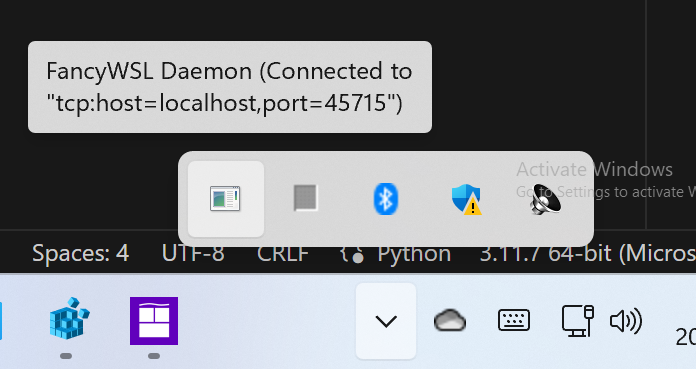
\includegraphics[width=0.5\linewidth]{assets/Screenshot 2023-12-20 114455.png}
    \caption{Hasil implementasi ikon status pada FancyWSL}
\end{figure}

\subsection{Pengimplementasian Fungsi Penanganan Notifikasi}

Pada pengimplementasian aspek penanganan notifikasi (\textit{notification handling}) tugas akhir ini, terdapat dua hal utama yang perlu dilakukan:
\begin{itemize}
    \item \textbf{Pembuatan layanan (\textit{service}) yang teregistrasi di bus perpesanan D-Bus dan bertugas menangkap notifikasi-notifikasi yang dikirim oleh perangkat-perangkat lunak Linux yang berjalan di WSL}\\
    Hal ini diimplementasikan pada berkas kode \path{services/notifications.py}. Mekanisme kode ini adalah dengan mengekspos metode "Notify()" pada perangkat lunak FancyWSL yang dapat dipanggil oleh perangkat-perangkat lunak di WSL yang ingin mengirimkan notifikasi dengan parameter-parameter yang berisi informasi notifikasi tersebut.

    \item \textbf{Penghubungan dengan API Windows yang menangani aspek penampilan notifikasi di \textit{shell} Windows}
    Pada perangkat lunak yang dikembangkan pada tugas akhir ini (FancyWSL), digunakan pula pustaka pemrograman pihak ketiga bernama \verb|winsdk| yang bertindak sebagai \textbf{binding} API Windows agar dapat diakses melalui program yang menggunakan bahasa pemrograman Python. Hal ini diimplementasikan pada berkas kode \path{shell/toast_notification.py}.
\end{itemize}

Secara garis besar, mekanisme penanganan notifikasi ini bekerja adalah dengan membentuk templat XML ToastNotification yang akan ditampilkan di Windows dan mensubstitusikan nilai-nilai yang ada dengan parameter-parameter yang didapat dari pemanggilan metode "Notify()" layanan FancyWSL oleh perangkat-perangkat lunak di WSL yang ingin mengirimkan notifikasi. Kode yang bersangkutan terlampir pada bagian lampiran.

\subsection{Pemgimplementasian Fungsi Kontrol Media}

Pengimplementasian aspek pengontrolan media pada FancyWSL melibatkan dua hal utama yang perlu dilakukan:
\begin{itemize}
    \item \textbf{Penangkapan sinyal-sinyal yang memberitahukan penggantian informasi media yang sedang diputar di bus perpesanan D-Bus}
    Hal ini diimplementasikan pada berkas kode \path{services/media_control.py}. Kode ini bekerja dengan cara
    \begin{enumerate}
        \item menambahkan aturan kecocokan (\textit{match rule}) tentang pengontrolan media (MPRIS) kepada pengelola bus perpesanan D-Bus atas nama perangkat lunak FancyWSL agar FancyWSL dapat menerima pesan-pesan yang memiliki kecocokan dengan aturan kecocokan tersebut (hal ini sesuai dengan spesifikasi D-Bus \cite{dbus-specification} dan diperlukan untuk alasan keamanan agar mengurangi kemungkinan terjadinya \textit{sniffing}),
        
        \item melakukan \textit{subscribe} pada bus perpesanan D-Bus yang terhubung dan menunggu pesan-pesan yang sesuai dengan aturan kecocokan di atas masuk, dan
        
        \item memproses pesan-pesan yang masuk tersebut dengan cara meneruskan ke modul \path{shell/smtc.py}.
    \end{enumerate}

    \item \textbf{Penghubungan dengan API Windows yang menangani aspek pengontrolan media universal}
    Hal ini diimplementasikan pada berkas kode \path{shell/smtc.py}. Mekanisme kode ini bekerja adalah dengan
    \begin{itemize}
        \item meneruskan properti-properti yang didapat dari sinyal yang ditangkap dari bus perpesanan D-Bus ke pemanggilan API SystemMediaTransportControls pada Windows dan
        
        \item memanggil metode-metode, seperti "PlayPause()", "Next()", "Previous()", dan "Stop()", pada objek \path{/org/mpris/MediaPlayer2} di D-Bus apabila terdapat interaksi dari pengguna seperti penekanan tombol putar/jeda, penekanan tombol \textit{next}, dan penekanan tombol \textit{previous}, pada panel pengontrolan media universal yang tampil di \textit{shell} Windows.
    \end{itemize}
\end{itemize}

\subsection{Pengimplementasian \textit{Guards} Tambahan}

Pada pengembangan perangkat lunak FancyWSL, diimplementasikan sejumlah \textit{guard} atau proteksi tambahan yang memastikan FancyWSL berjalan pada platform yang semestinya, mencegah/menghalangi penjalanan FancyWSL pada platform yang tidak berhubungan sama sekali (seperti macOS), dan memastikan bahwa kapabilitas-kapabilitas pada WSL yang diperlukan untuk bekerjanya FancyWSL tersedia, aktif, dan dapat diakses. Seluruh \textit{guard} yang diimplementasikan terletak pada berkas kode \path{helpers/verify_platform.py}. Berikut \textit{guard}-\textit{guard} yang diimplementasikan pada FancyWSL.

\begin{itemize}
    \item Pemastian bahwa sistem operasi tempat FancyWSL dijalankan adalah Windows (di luar WSL), bukan platform lain atau di dalam WSL (\verb|_verify_proper_os()|)
    
    \item Memastikan bahwa perangkat lunak WSL telah terinstal dengan baik di \textit{host} Windows (\verb|_verify_wsl_availability()|)
    
    \item Pemeriksaan bahwa distribusi \textit{default} pada WSL merupakan WSL versi 2 (WSL2) yang telah mendukung sistem init systemd dan perangkat-perangkat lunak berantarmuka grafis (GUI) (\verb|_verify_wsl_availability()|)
    
    \item Memeriksa bahwa sistem init systemd tersedia dan telah aktif pada distribusi WSL yang akan digunakan (\verb|_verify_wsl_availability()|)
\end{itemize}

Seluruh fungsi \textit{guard} di atas bersifat privat (\textit{private function}) dan hanya tersedia untuk diakses pada modul tersebut; hanya terdapat satu fungsi tunggal, \verb|verify_platform()|, yang menggabungkan fungsi-fungsi \textit{guard} di atas dan diekspos kepada modul-modul luar yang memanfaatkan modul ini.

\section{Pengintegrasian FancyWSL dengan \textit{Lifecycle} Windows Subsystem for Linux (WSL)}

Perangkat lunak FancyWSL yang telah dikembangkan dapat dijalankan secara manual setiap kali pengguna ingin merasakan tingkat integrasi WSL dengan Windows yang lebih mendalam. Namun, mengingat solusi ini berkaitan dengan integrasi yang umumnya bersifat transparan ke pengguna, akan jauh lebih baik apabila fungsionalitas integrasi yang ditingkatkan ini berjalan secara mandiri dan otomatis. Hal ini dapat dicapai salah satunya dengan menambahkan perangkat lunak FancyWSL sebagai layanan (\textit{service}) systemd.

Untuk mengimplementasikan hal ini, dibuat sebuah berkas baru yang terletak di \path{/home/<nama-pengguna>/.config/systemd/user/fancywsl-windows-daemon.service} yang digunakan sebagai defisi layanan (\textit{service}) FancyWSL. Berkas tersebut berisi informasi-informasi penjalanan perangkat lunak FancyWSL sebagai layanan \textit{service} systemd. Berikut isi berkas tersebut.

\begin{lstlisting}
[Unit]
Description=FancyWSL Windows-side daemon
After=dbus.service

[Service]
ExecStart=/home/comfyte/.local/bin/start-fancywsl-windows-daemon.sh

[Install]
WantedBy=graphical.target
\end{lstlisting}

Berdasarkan berkas definisi tersebut, layanan (\textit{service}) systemd ini akan dijalankan setelah layanan D-Bus berjalan. Berkas ini juga menginstruksikan agar layanan ini menjalankan sebuah berkas \textit{shell script} yang terletak di \path{/home/comfyte/.local/bin/start-fancywsl-windows-daemon.sh}. Berikut isi berkas \textit{shell script} tersebut.

\begin{lstlisting}[language=bash]
#!/usr/bin/env bash
export BUS_ADDRESS_FOR_FWSL=$(journalctl --user -b -u dbus.service | grep 'dbus-daemon' | tail -n 1 | grep -P -o 'tcp\:host=\S+,port=\d+(?:,family=(?:ipv4|ipv6))?')
export PYTHONPATH=/mnt/c/Users/rafir/Projects/skripsi/FancyWSL
WSLENV=$WSLENV:PYTHONPATH/wp /mnt/c/Users/rafir/AppData/Local/Microsoft/WindowsApps/python3.exe -m fwsl_daemon --bus-address="$BUS_ADDRESS_FOR_FWSL"
\end{lstlisting}

Dalam isi berkas \textit{shell script} tersebut, terdapat penjalanan berkas \textit{executable} berakhiran \verb|.exe| secara langsung di dalam lingkungan Linux (WSL). Hal ini dimungkinkan oleh kemampuan WSL dalam menjalankan berkas \textit{executable} Windows secara langsung di dalam lingkungan WSL \cite{msdocs-run-windows-tools-from-linux}.

\section{Dokumentasi Pengujian Akhir FancyWSL}

\begin{figure}[H]
    \centering
    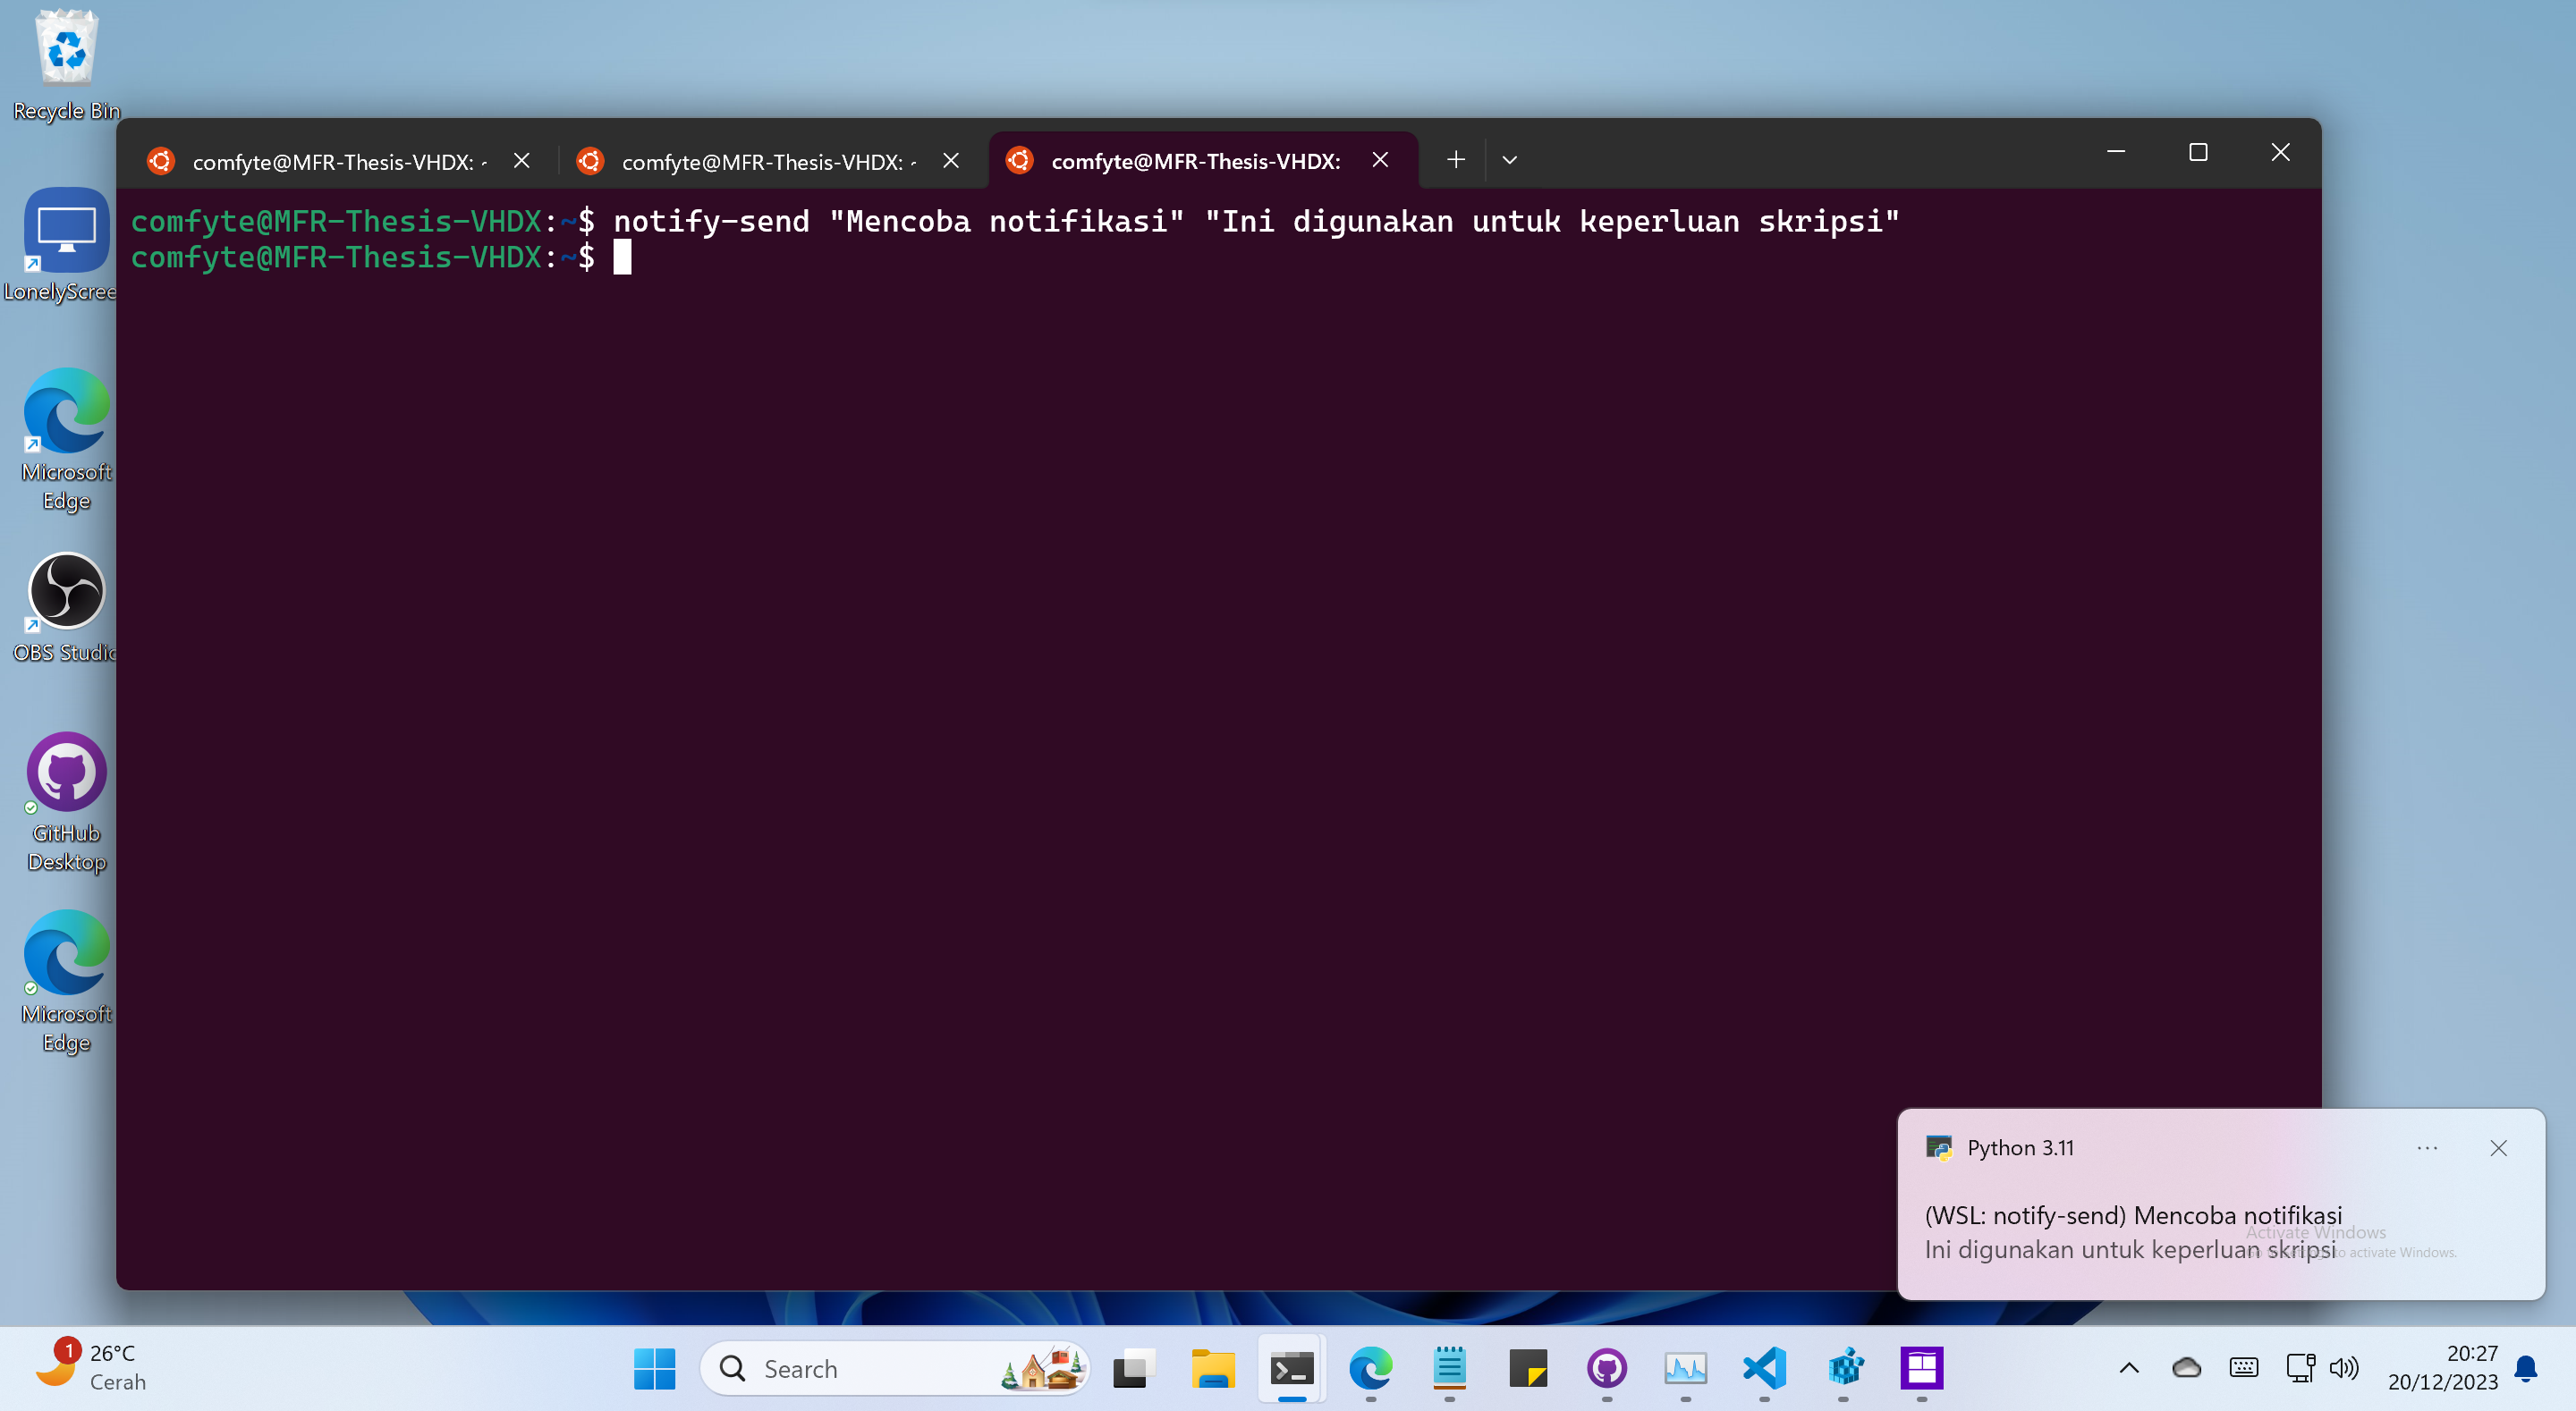
\includegraphics[width=1\linewidth]{assets/Screenshot 2023-12-20 202713.png}
    \caption{Fungsionalitas notifikasi saat ini bekerja pada perangkat lunak yang berjalan di dalam WSL saat \textit{daemon} FancyWSL dijalankan.}
    \label{fig:enter-label}
\end{figure}

\begin{figure}[H]
    \centering
    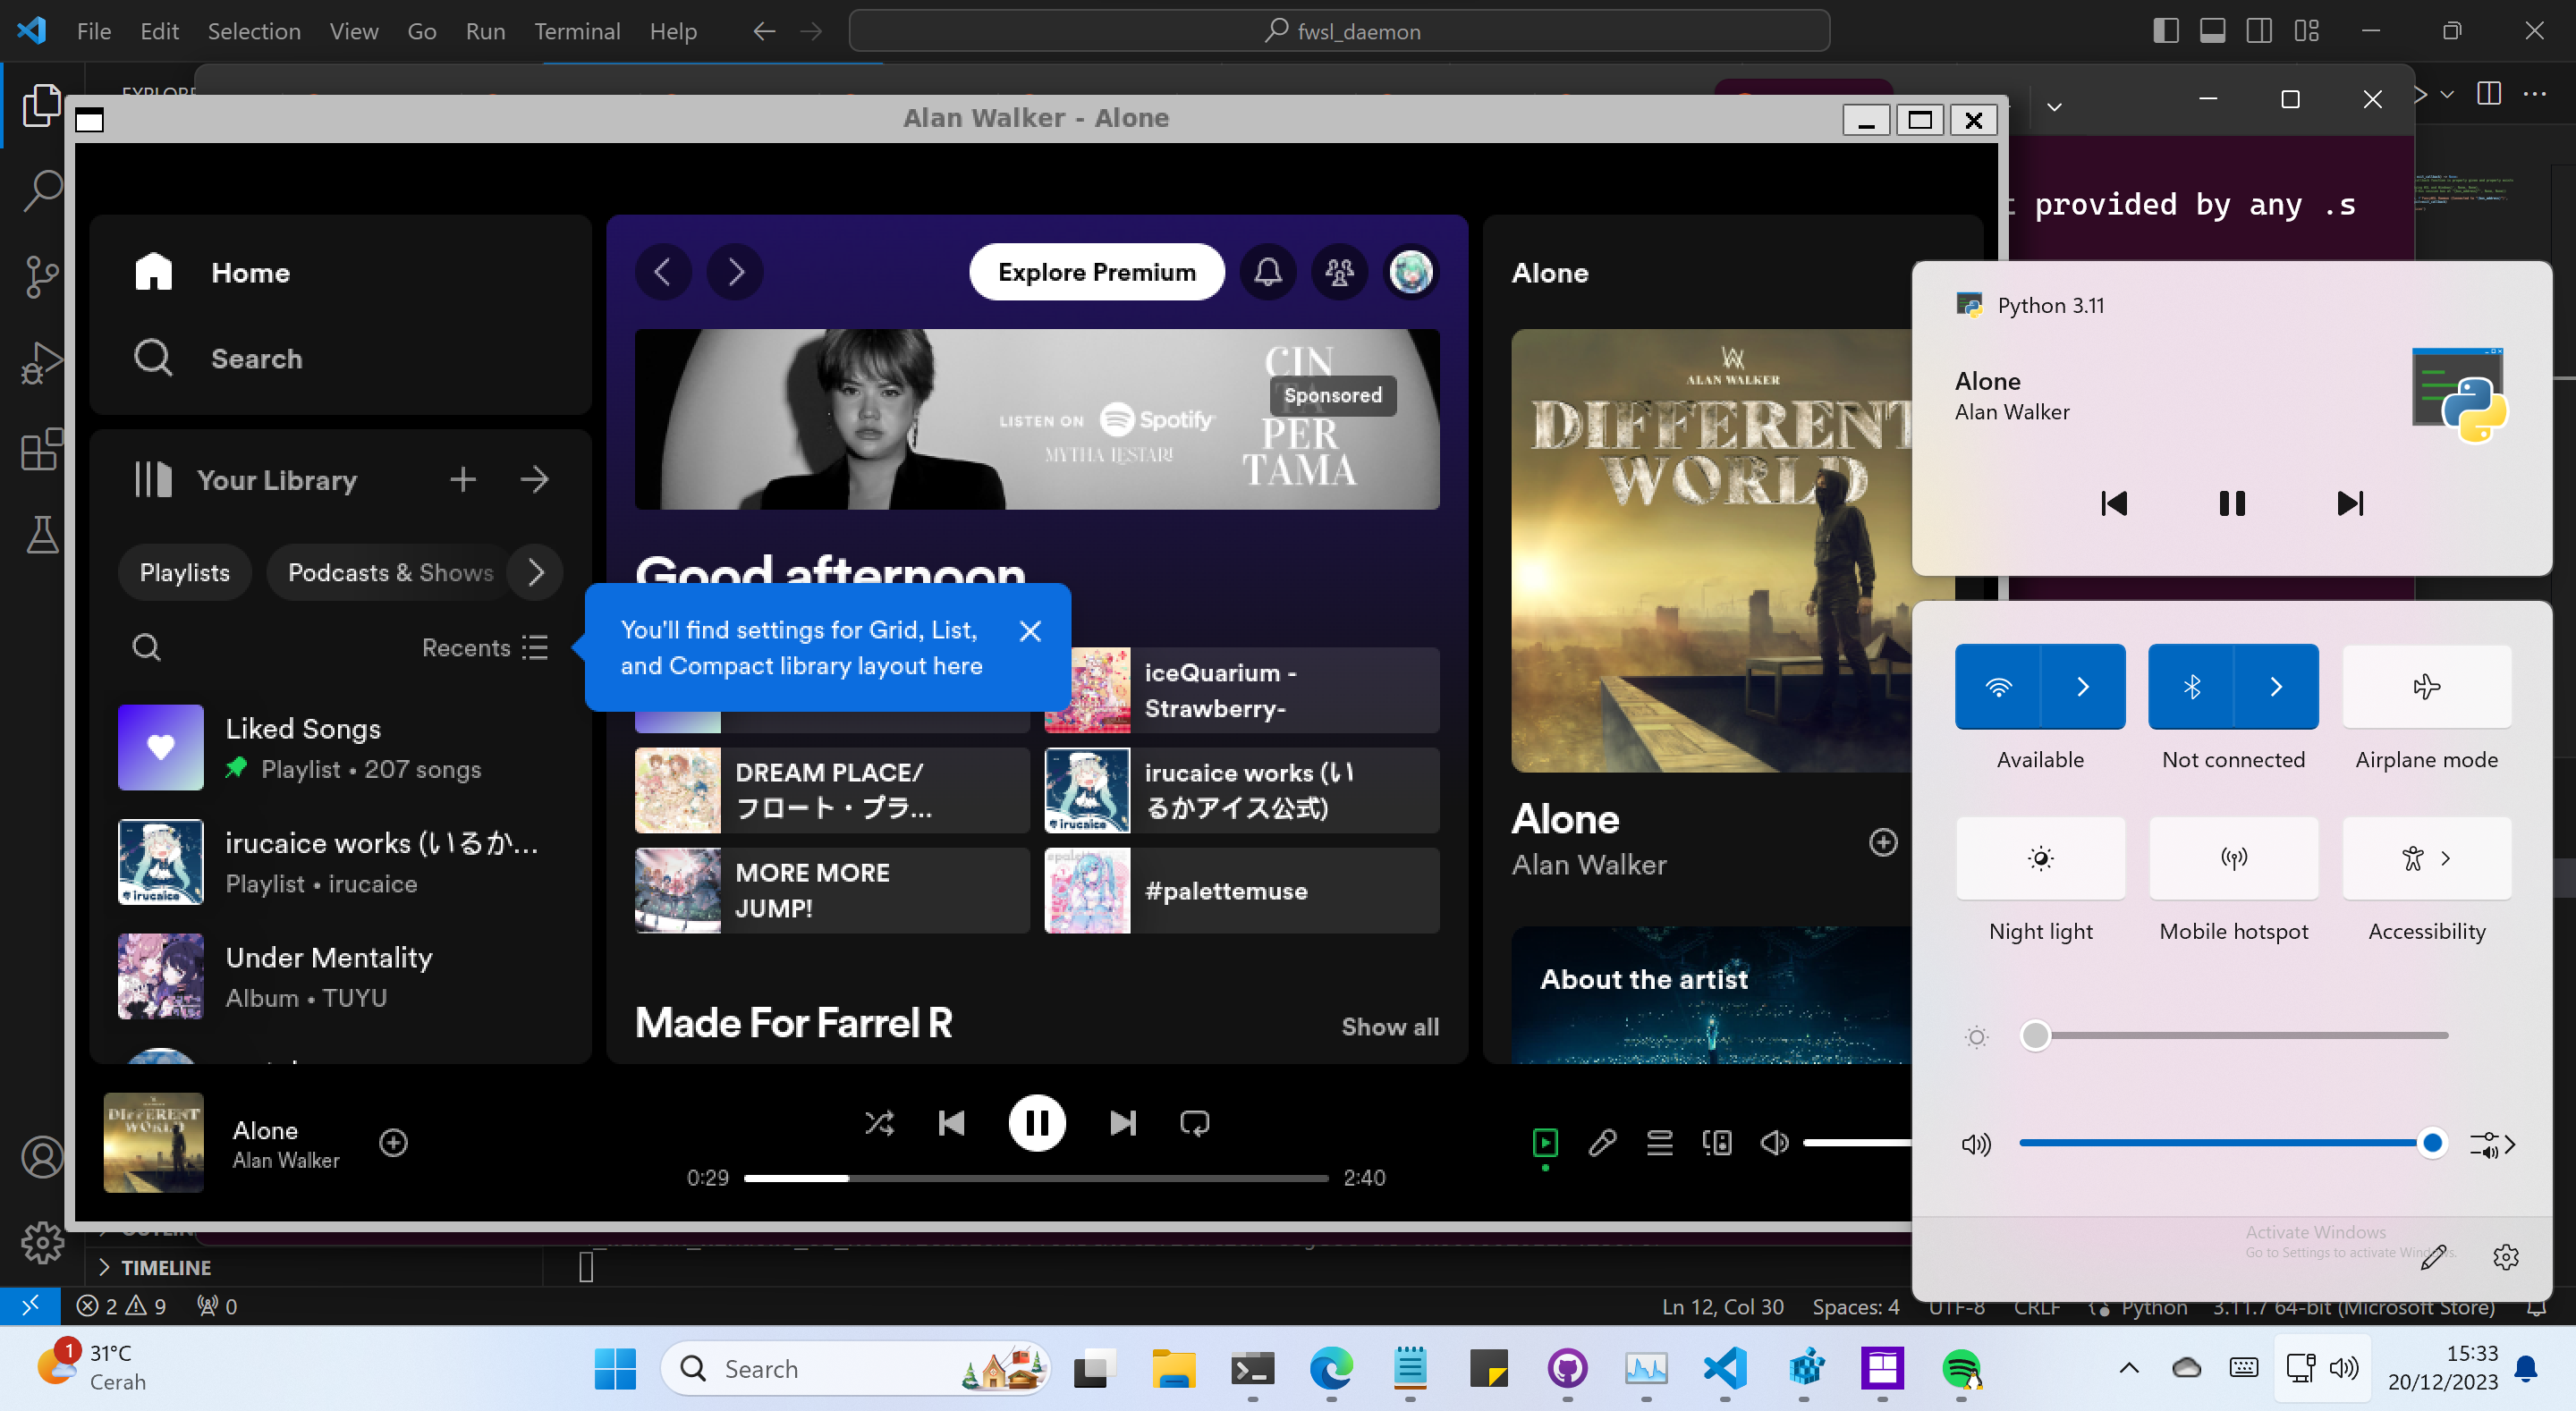
\includegraphics[width=1\linewidth]{assets/Screenshot 2023-12-20 153317.png}
    \caption{Fungsionalitas kontrol media saat ini bekerja pada perangkat lunak yang berjalan di dalam WSL saat \textit{daemon} FancyWSL dijalankan.}
    \label{fig:enter-label}
\end{figure}

\section{Kelebihan dan Kekurangan Solusi pada Tugas Akhir Ini}

\subsection{Kelebihan}

\begin{enumerate}
    \item Perangkat lunak FancyWSL memungkinkan pengintegrasian, dua hal yang sebelumnya belum bisa dilakukan.
    \item FancyWSL menggunakan kemampuan bawaan D-Bus dalam berkomunikasi menggunakan protokol TCP, sehingga proses komunikasi berlangsung cukup efisien dibandingkan dengan metode-metode lain yang telah disebutkan pada Bab II.
    \item FancyWSL bersifat mandiri dan dapat berjalan secara otomatis pada saat suatu \textit{instance} WSL dijalankan (hasil integrasi dengan sistem init systemd) dan dapat menutup secara otomatis saat tidak ada \textit{instance} WSL lagi yang berjalan (ketiadaan koneksi dengan bus perpesanan D-Bus akan mengakhiri \textit{main loop} pada FancyWSL sehingga menutup FancyWSL secara otomatis).
\end{enumerate}

\subsection{Kekurangan}

\begin{enumerate}
    \item Fungsi penampilan notifikasi pada FancyWSL masih terbatas pada penampilan notifikasi sederhana tanpa ikon, pengaturan durasi penampilan notifikasi, dan aksi-aksi tambahan seperti tombol.

    \item Fungsi pengontrolan media masih bersifat \textit{buggy} dan terkadang tidak bekerja karena berbagai alasan. Selain itu, informasi media yang ditampilkan belum memunculkan elemen-elemen tambahan seperti gambar album.
\end{enumerate}

% \section{Perbandingan Hasil Penelitian dengan Hasil Terdahulu}

% Sejauh ini, baru terdapat satu buah penelitian dahulu yang membahas topik yang sama dengan tugas akhir ini, yakni tesis master berjudul
